\section*{Overview}
The advent of several parallel programming models such as CUDA\footnote{Parallel computing platform and programming model invented by NVIDIA} and OpenCL\footnote{Framework for writing programs that execute across heterogeneous platforms such as GPUs}, provided us with the tools that can be used to write heavy computational programs which utilizes the multi-threaded power of the GPUs. Yuan and others started research on utilizing this power of GPU to process data warehousing queries, typically OLAP workloads. They believed that the implementation of such database system with the acceleration of the GPU, can provide extremely high-throughput as compared to the CPU or other processing engines.
\newline
They build several modules using the drivers and libraries provided by CUDA and OpenCL to implement a database system called GPUDB\cite{gpudb_design_impl}, which enabled them to execute OLAP workload driven queries on the GPU and evaluate performance of the system by benchmarking it with the SSBM queries, as performed by CoGaDB.

\section*{Architecture}
The architecture of GPUDB is shown in figure \ref{fig:gpudbarch}. As the most DBMSs, GPUDB follows the same approach of providing SQL client interface for the user to submit queries. This input query is then passed to SQL parser which converts the provided query into logical query plan. It is then followed by query optimizer, which implements in-built optimizations routines on the logical query plan for efficient transformation. Both parser and query optimizer is built upon the same coding strategy as shown by the Lee and others with their SQL to MapReduce translator called YSmart\footnote{Yet Another SQL-to-MapReduce Translator}. This approach provides efficient algorithms to transform SQL-like queries into map-reduce jobs, which can be run in distributed environments very efficiently.

\begin{figure}[ht]
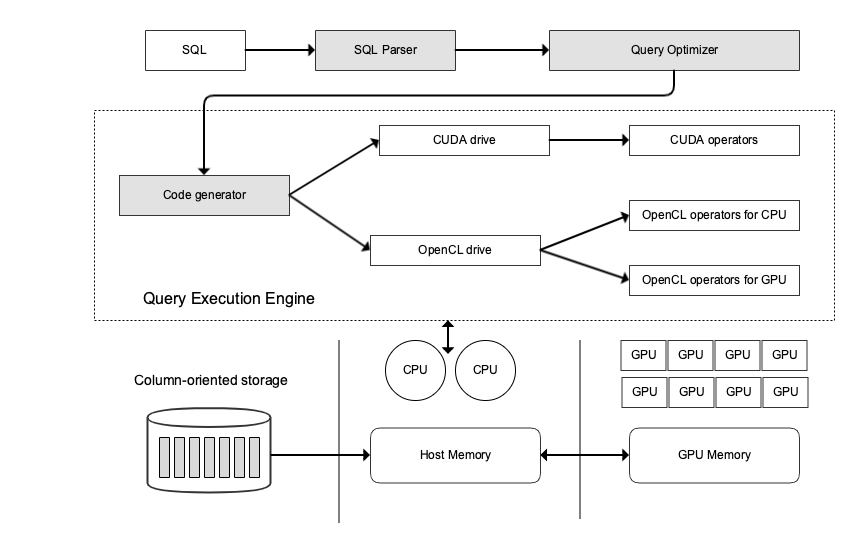
\includegraphics[width=15cm,height=15cm,keepaspectratio]{gpudb/gpudb_architecture.png}
\caption{The architecture of GPUDB, taken from \cite{gpudb_design_impl}}
\label{fig:gpudbarch}
\end{figure}

The optimized logical query plan is then provided to query execution engine of GPUDB for generating machine code variant that can be executed on the GPU kernels. The execution engine consists of code generator with CUDA and OpenCL pre-implemented operators which helps in execution of query plan operators inside GPU space. The engine's code generator can generate either CUDA or OpenCL code variant and induce operators depending upon the selected processing environment. The engine adopts a push-based, block-oriented execution model which executes the provided query plan in post-order sequence\cite{gpudb_design_impl} with block-oriented execution. It manages GPU memory for the operator's execution and tries to keep as much data in GPU memory as possible for efficient operator's processing.
\newline
Column-oriented storage is used by the system as the backend store, which is extremely efficient for OLAP workloads due to its efficiency of storing data in columnar manner. The engine relies on the late materialization strategy\cite{gpudb_materialization}, which fetches the required columns by the operators into the memory at the very end of the processing. This strategy lazily loads the columns into memory depending upon the requirements which increases the performance of the system. Furthermore, some of the code is executed in the CPU kernels which handles the data transfer between CPU's host memory to GPU's memory and initiating GPU kernels whenever required.

\section*{Exploring the design-space}
In this section, we discuss the design-space of GPUDB using functional and non-functional properties. We have researched and performed in-depth analysis of the GPUDB on 8 different parameters which are stated below.

\section*{Functional properties}
In the following, we perform analysis on the functional properties on which DBMSs are designed upon. We target underlying storage and processing models of GPUDB, how query optimisation and consistency is achieved in the system and researched several other aspects to understand its functional nature.

\section*{Storage system}
The limited amount of speed attained by PCIe\footnote{Peripheral Component Interconnect express(PCIe) - interface for connecting high-speed components} data transfer is one of the major bottleneck of the GPU architecture. Due to this limitation, GPU-accelerated databases suffer major performance hits since they need data to be stored in GPU memory. Yuan and others have identified solution to this limitation by introducing a crucial optimization concept of pinned host memory, which is a memory that cannot be swapped out leading to allowance of direct access by the GPUs.

Initially, GPUDB loads the entire database into CPU's host memory in order to avoid disk transfer bottlenecks, which is similar to CoGaDB. Futhermore, GPUDB stores some of the data in pinned host memory depending upon the operators and query plan, which is directly accessible by the GPU. This optimization avoids the major transfer bottleneck of CPU's host memory to GPU transfer using slow PCIe bus, leading to extremely improved performance.

\section*{Storage Model}
GPUDB is implemented with the objective of giving optimal performance with data warehousing workloads. The system is required to adapt to such storage model which can increase its efficiency in transferring data with late materialization strategy and can be compressed easily to avoid major transfer bottlenecks.

Taking all these requirements into consideration, GPUDB adopted column-oriented storage as their primary storage model due to its extreme efficiency in supporting compression algorithms and materialization strategy. GPUDB's query engine supports three data compression techniques which is very effective and easy to implement in columnar storage: Run Length Encoding(RLE), Bit Encoding and Dictionary Encoding\cite{gpudb_design_impl}. Wang and others have shown that significant performance improvements can be obtained using graphics processors when worked with compressed data\cite{gpudb_fast_computations}. Thus, GPUDB directly works with the compressed data for performing computations and operations whenever possible, which is supported by using column-oriented storage model.

\section*{Processing Model}
AS shown in Figure \ref{fig:gpudbarch}, GPUDB provides SQL client interface and interactive component for users to push their SQL queries to the database engine. For processing these queries, GPUDB uses a block-oriented processing model\cite{gpudb_block_processing}, which is a technique in which operators are processed in blocks as compared to singleton operators processing as represented in the figure \ref{fig:gpudb_processing_models}.

\begin{figure}[ht]
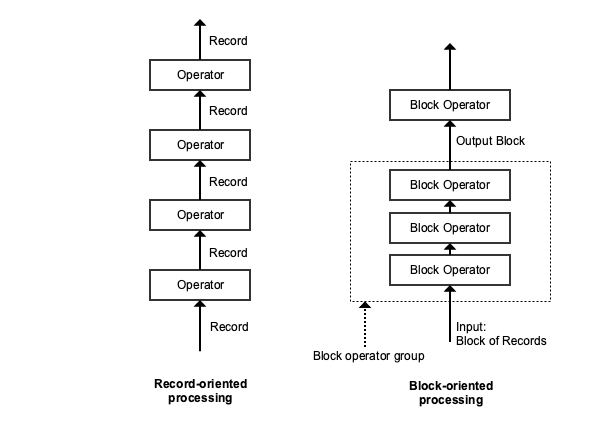
\includegraphics[width=15cm,height=15cm,keepaspectratio]{gpudb/block_processing_model.png}
\caption{Processing models strategies, taken from \cite{gpudb_block_processing}}
\label{fig:gpudb_processing_models}
\end{figure}

GPUDB implements this block-oriented processing by keeping blocks of operators in GPU memory until they are completely processed. This processing model is further boosted by the support of pre-implemented GPU operators provided by the code generation to CUDA or OpenCL driver programs. Due to this, GPUDB executes all its operations on the GPU and use CPU's host memory for managing data transfer requirements and completing post processing tasks.

\section*{Buffer Management}
Unlike CoGaDB, GPUDB does not provide any dedicated buffer management module for implementing efficient data placement strategies. It handles its data requirements by running an isolated program interface on the host CPU's main memory which fetches data from column-oriented storage to provide it to GPU memory in late materialization manner. This program also handles data placement in host's pinned memory for enable direct access by the GPU. This system is responsible for ensuring data availability to the operations running in the GPU environment.

\section*{Query placement and optimizations}
GPUDB does not implement any processor selection and cost estimation algorithm to decide query placements depending upon the requirement. It only supports the execution of any database related operations in the GPU environment using CUDA or OpenCL driver programs which are designed and optimized with pre-implemented GPU operators. The query engine cannot execute any operation in another co-processor environment, unlike CoGaDB, which does this task using its Hybrid Query Processing Engine(HyPE).
GPUDB supports optimizations using its query optimizer module which induces certain performance improving changes in the logical query plan using provided algorithms and strategies. Furthermore, query engine adds more optimizations in the query plan while transforming it into CUDA or OpenCL driver programs.

\section*{Consistency and Transaction Processing}
GPUDB does not implement any algorithms or strategies for maintaining consistency standards for the system. After reviewing and reading several research papers, it can be concluded that GPUDB does not provide any fault tolerance policies or locking mechanism for handling transactions or inconsistency in the system. The query engine is entirely focused on processing and executing query operators to produce results with the best performance. There is no module with the implementation of consistency and transaction processing in the GPUDB ecosystem.

\section*{Non-Functional Properties}
In the following, we perform analysis on the non-functional properties for which DBMSs are typically optimized and tweaked upon. We target performance and portability as the parameters of understanding GPUDB non-functional nature.

\section*{Performance}
Yuan and others benchmarked and analyzed performance of GPUDB by using Star Schema Benchmarking (SSBM) queries to simulate OLAP workloads. They also performed analysis of using pageable and pinned host memory for understanding the complications and limitations of PCI express bus data transfer. These performance insights can be visualized in the Figure \ref{fig:ssbm_gpudb}.

\begin{figure}[htb]
    \centering % <-- added
\begin{subfigure}{0.5\textwidth}
  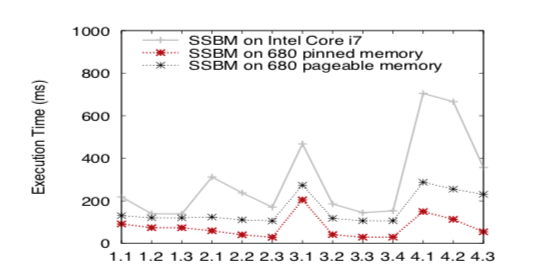
\includegraphics[width=\linewidth]{gpudb/cpu_vs_gpu.png}
\end{subfigure}\hfil % <-- added
\begin{subfigure}{0.5\textwidth}
  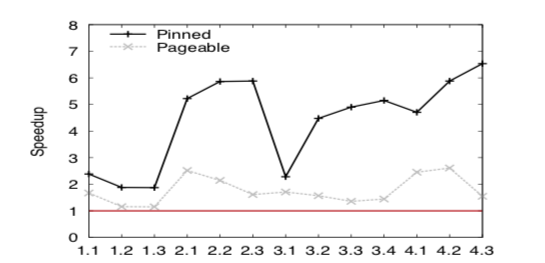
\includegraphics[width=\linewidth]{gpudb/pinned_vs_pageable}
\end{subfigure}\hfil % <-- added
\caption{SSBM performance comparison, taken from \cite{gpudb_design_impl}}
\label{fig:ssbm_gpudb}
\end{figure}

From the performance insights, it can be clearly concluded that GPUDB provides better performance for OLAP workloads as compared to CPU driven architecture. Furthermore, the results of using pinned memory clearly provides us the implication that PCI express data transfer bottleneck hampers performance of the GPU-accelerated database systems. Hence, GPUDB can be considered as a suitable high performing GPU-accelerated database system for managing and processing data warehousing workloads.

\section*{Portability}
GPUDB is extremely dependent on NVIDIA's CUDA libraries and OpenCL framework support providing graphics card. From this perspective, GPUDB fulfill very limited hardware-oblivious requirements as it did not implement all vendor-specific operators which are currently available in several heterogeneous processing environments. Due to this, GPUDB leads to comparatively less development and implementation costs but approaches towards more hardware-aware design paradigm. In terms of portability perspective, GPUDB needs to incorporate lots of module and vendor-specific changes in order to become hardware-oblivious.